%%%%%%%%%%%%%%%%%%%%%%%%%
\section{Experimental results}
\label{sect:experiment}

In this section we demonstrate that the mixing time of the proposed method, 
\emph{augmented Gibbs} sampling, is faster than Rejection sampling, baseline 
Gibbs and Metropolis-Hastings.     
Algorithms are tested against two different models. The BPPL model of Example~\ref{example:pref} and a \emph{Market maker} (MM) model motivated by \cite{Das:08}:

\begin{figure}
\centering
\begin{subfigure}{.35\textwidth}
\centering
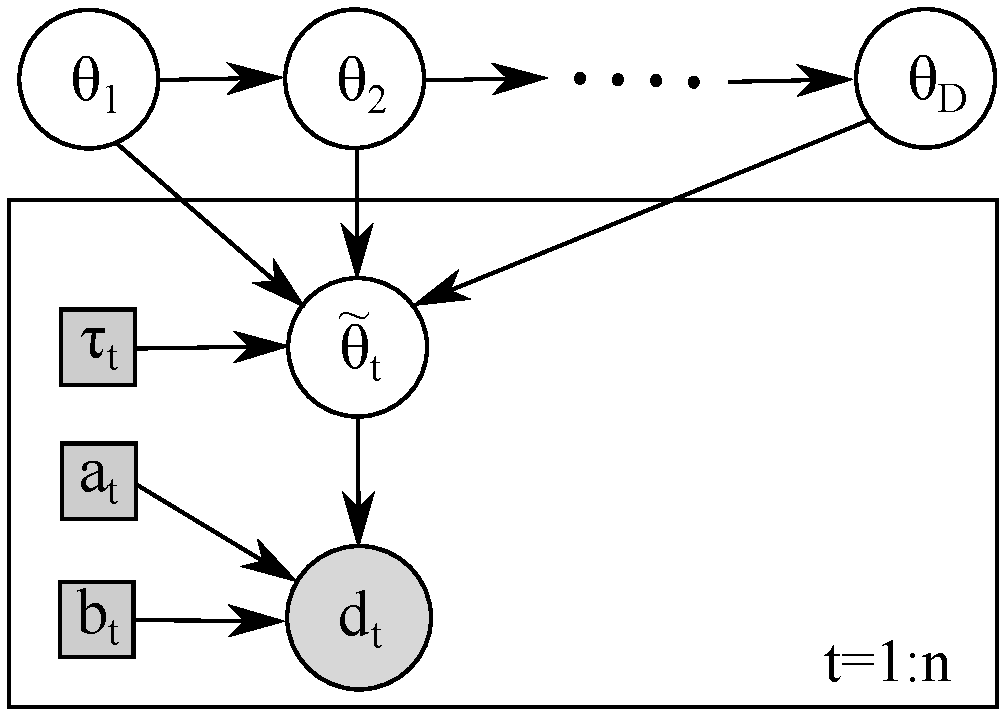
\includegraphics[width=.90\textwidth]{pic/market4w.pdf}
%\vspace{-6mm}
\caption{}%\footnotesize Market maker model using plate notation. }
\label{fig:market}
\end{subfigure}
\begin{subfigure}{.24\textwidth}%\vspace{2mm}
  \centering
  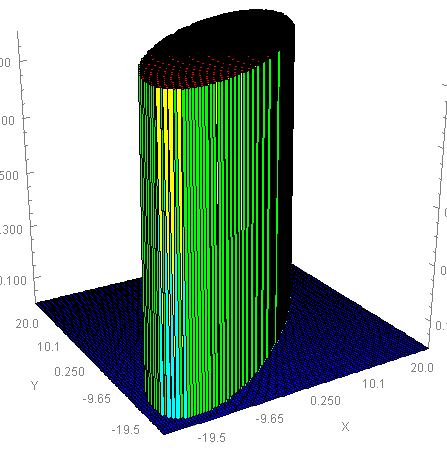
\includegraphics[width=.82\textwidth]{pic/elipsePrior.png}
  \caption{}
  \label{fig:mmm.prior}
\end{subfigure}%
\begin{subfigure}{.24\textwidth}%\vspace{8mm}
  \centering
  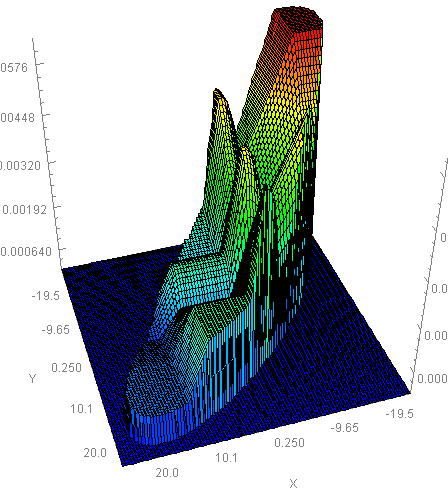
\includegraphics[width=.8\textwidth]{pic/MM2.png}
  \caption{}
  \label{fig:mmm.posterior}
\end{subfigure}
\caption{\footnotesize Instrument type value distribution of Market Maker problem of Example~\ref{example:market}.
(a) prior, (b) posterior given 4 observed data points (trader responses).}
\label{fig:mmm}
\end{figure}
%%%%%%%%%%%%%%%%%%%%%%%
\vspace{1mm}
\fexample{example:market}{Market maker (MM)}{
Suppose there are $D$ different types of \emph{instruments} with 
respective valuations 
$\boldsymbol\theta=\{\boldsymbol\theta_{1}\ldots\boldsymbol\theta_{D}\}$.
There is a \emph{market maker} 
who at each time step $t$ deals an instrument of type $\tau_t \in \{1, 
\ldots D\}$ by setting \emph{bid} and \emph{ask} $b_{t}$ and $a_{t}$ denoting 
prices at which she is willing to buy and sell each unit respectively 
(where $b_{t} \leq a_{t}$).
The ``true" valuation of different types
are unknown (to her) but any a priori knowledge over their dependencies that can be expressed via a DAG structure over their associated random variables is permitted.
Nonetheless, without loss of generality we only consider the following simple dependency:  
Assume the types indicate different versions of the same product and
each new version is more expensive than the older ones ($\boldsymbol\theta_{i} 
\leq 
\boldsymbol\theta_{i+1}$).
The valuation of the oldest version is within some given price range $[L, H]$
and the price difference of any consecutive versions is bound by a known parameter $\delta$:
\begin{align*}
pr(\boldsymbol\theta_{1}) & = \mathcal{U}(L, H) \qquad \qquad\\
pr(\boldsymbol\theta_{i+1}) & = \mathcal{U}(\boldsymbol\theta_{i}, 
\boldsymbol\theta_{i} + \delta) \quad \forall i \in \{1, \ldots, D-1\}
\end{align*} 
At each time-step $t$, a trader arrives. 
He has a noisy estimation $\widetilde{\boldsymbol\theta_{t}}$ of the actual 
value of the presented instrument $\tau_t$. 
We assume 
$pr(\widetilde{\boldsymbol\theta_{t}} | \, \boldsymbol\theta, \, \tau_t = i) = 
\mathcal{U}(\boldsymbol\theta_{i} - \epsilon, \boldsymbol\theta_{i} + 
\epsilon)$.
The trader response to bid and ask prices 
$a_{t}$ and $b_{t}$ is $d_t$ in $\{\textsc{Buy}, \textsc{Sell}, \textsc{Hold}\}$. 
If he thinks the instrument is undervalued by the ask price (or overvalued by the bid price), with probability 0.8, he will buy it (resp. sell it), otherwise holds. 
\begin{align*}
pr (\textsc{Buy} \, | \, \widetilde{\boldsymbol\theta_{t}}, a_{t}, b_{t}) &=
{\footnotesize
\begin{cases}
\widetilde{\boldsymbol\theta_{t}}  <     a_{t} 		: 0\\
\widetilde{\boldsymbol\theta_{t}}  \geq a_{t}  		: 0.8
\end{cases}
}
&\\
pr (\textsc{Sell} \, | \, \widetilde{\boldsymbol\theta_{t}} , a_{t}, b_{t}) &= 
{\footnotesize
\begin{cases}
\widetilde{\boldsymbol\theta_{t}} \leq b_{t} 		: 0.8\\
\widetilde{\boldsymbol\theta_{t}} > b_{t} 		: 0
\end{cases}
}
\\
pr (\textsc{Hold} \, | \, \widetilde{\boldsymbol\theta_{t}}, a_{t}, b_{t}) &=
{\footnotesize
\begin{cases}
b_{t} < \widetilde{\boldsymbol\theta_{t}} < 
a_{t} 								 & : 1\\
\widetilde{\boldsymbol\theta_{t}} \leq b_{t} \, \vee\,  
\widetilde{\boldsymbol\theta_{t}} 
\geq a_{t}	 	 & : 0.2
\end{cases}
}
\end{align*}
Based on traders' responses, the market maker intends to compute the posterior distribution of the valuations of all instrument types.
To transform this problem (with corresponding model shown in 
Figure~\ref{fig:market})
to the model represented by Equation~\ref{e:posterior}, variables 
$\widetilde{\boldsymbol\theta_{t}}$ should be marginalized.
For instance:
{\footnotesize
\begin{eqnarray}
{\footnotesize
pr(\textsc{Buy} \, | \, \boldsymbol\theta, a_{t}, b_{t}, \tau_t) \!\!\!\!\!\! 
}
&=&\!\!\!\!\!\! 
\int_{-\infty}^{\infty} pr(\textsc{Buy} \, | \, 
\widetilde{\boldsymbol\theta_t}, a_{t}, b_{t})
\cdot pr (\widetilde{\boldsymbol\theta_t} \, | \, \boldsymbol\theta, \tau_t ) d 
\widetilde{\boldsymbol\theta_t} 
\nonumber 
\\
&=&\!\!\!\!\!\! \int_{-\infty}^{\infty}
{\footnotesize
\!
\begin{cases}
\widetilde{\boldsymbol\theta_t}  		<     a_{t}  : 0\\
\widetilde{\boldsymbol\theta_t}  		\geq a_{t}  : 0.8
\end{cases} 
}
\nonumber 
\\
&& \qquad 
\otimes
{\footnotesize
\begin{cases}
\theta_{\tau_t} \!-\! \epsilon \leq \widetilde{\boldsymbol\theta_t} \leq 
\theta_{\tau_t} \!+\! \epsilon 					: \frac{1}{2 \epsilon} \\
\widetilde{\boldsymbol\theta_t} \!<\! \boldsymbol\theta_{\tau_t} \!-\! \epsilon 
\, \vee \, \widetilde{\boldsymbol\theta_t} \!>\! \boldsymbol\theta_{\tau_t} 
\!+\! \epsilon 	: 0  
\end{cases}
}
\!\!\!\!\!
d \widetilde{\boldsymbol\theta_t}
\nonumber \\
&=&\!\!\!\!\!\!
{\footnotesize
\begin{cases}
\boldsymbol\theta_{\tau_t} \leq a_{t} - \epsilon: 0\\
a_{t} \!-\! \epsilon < \boldsymbol\theta_{\tau_t} \leq a_{t} \!+\! \epsilon: 
0.4(1 \!+\! \frac{\boldsymbol\theta_{\tau_t} - a_t}{\epsilon})\\
\boldsymbol\theta_{\tau_t} > a_{t} + \epsilon : 0.8
\end{cases}
}
\end{eqnarray}
}}% end MM example

Models are configured as follows: In BPPL, $\eta = 0.4$ and \emph{prior} is uniform in a hypercube.
In MM, $L = 0$, $H=20$, $\epsilon = 2.5$ and $\delta=10$. 


%%%%%%%%%%%%%%%%%%%%%%%%%
%%%%%%%%%%%%%%%%%%%%%%%%%
\begin{figure*}[tb!]
\centering
\vspace{-5mm}
\begin{subfigure}{.48\textwidth}
  \centering
  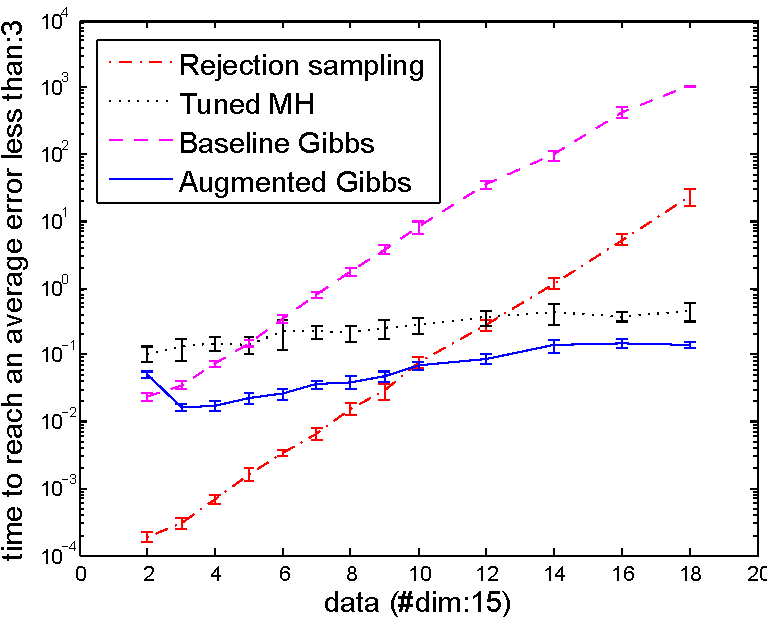
\includegraphics[scale=0.55]{plot/bppl_data_analysis_fit.pdf}
  \caption{}
  \label{fig:error-samples-bppl}
\end{subfigure}
\begin{subfigure}{.48\textwidth}
  \centering
  \hspace{5mm} 
  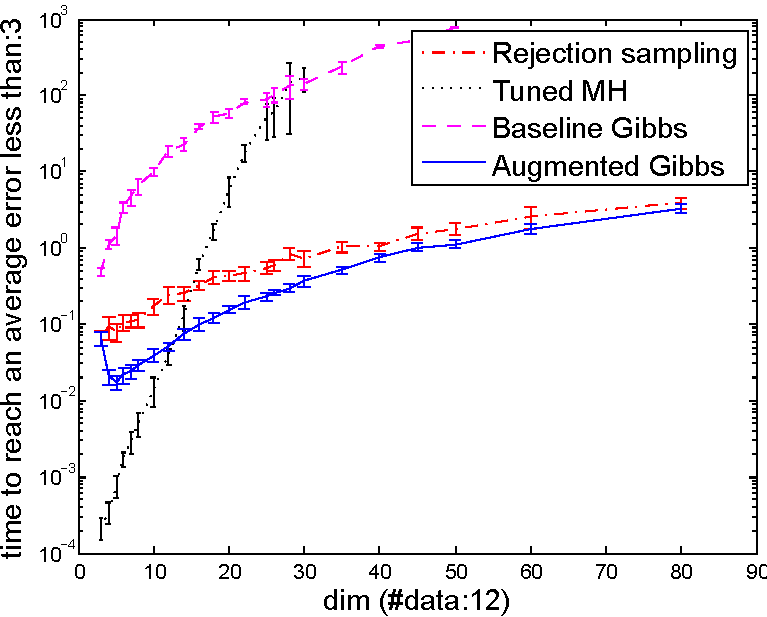
\includegraphics[scale=0.55]{plot/bppl_dim_analysis_fit.pdf}
  \caption{}
  \label{fig:error-samples-bppl}
\end{subfigure}
%\caption{Performance of Rejection/Metropolis-Hastings, baseline and augmented Gibbs on (a) \& (b) BPPL and (c) \& (d) MM models against different configurations of the number of observed data and the dimensionality of the parameter space.}
%\label{fig:results1}
%\end{figure}
%
%\begin{figure}[thbp!]
\centering
\begin{subfigure}{.48\textwidth}
  \centering
  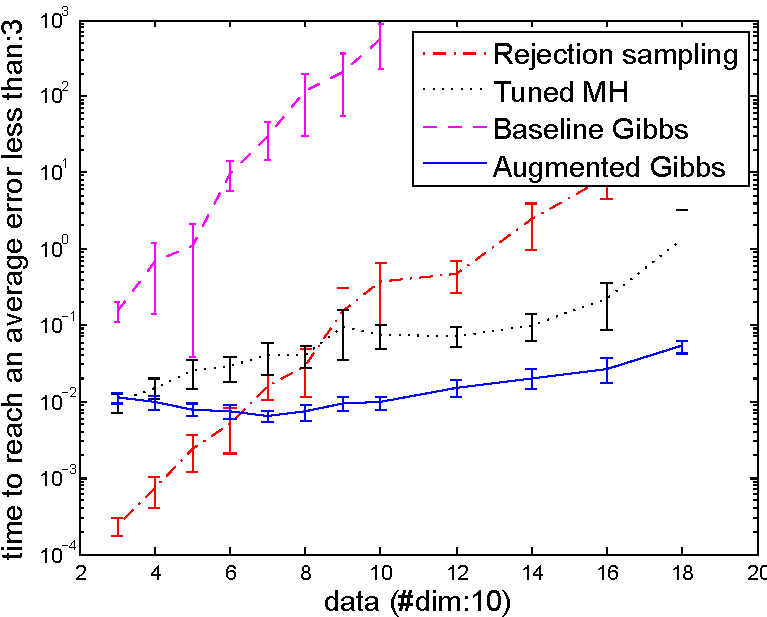
\includegraphics[scale=0.55]{plot/mmm_data_analysis2.pdf}
  \caption{}
  \label{fig:mmm_data_analysis}
\end{subfigure}
\begin{subfigure}{.48\textwidth}
  \centering
  \hspace{5mm} 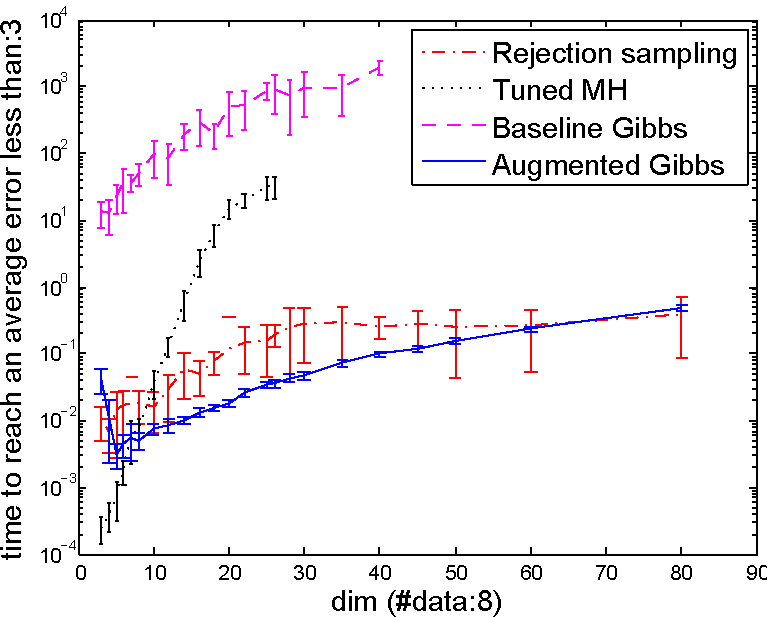
\includegraphics[scale=0.55]{plot/mmm_dim_analysis10.pdf}
  \caption{}
  \label{fig:mmm_dim_analysis}
\end{subfigure}
\vspace{-1mm}
\caption{\footnotesize Performance of Rejection/Metropolis-Hastings, baseline and augmented Gibbs on (a) \& (b) BPPL and (c) \& (d) MM models against different configurations of the number of observed data and the dimensionality of the parameter space.  In almost all cases, Augmented Gibbs takes orders of magnitude less time to achieve the same error as the other methods and this performance separation from competing algorithms increases in many cases with both the amount of data and dimensionality.}
\label{fig:results}
\vspace{-3mm}
\end{figure*}




For each combination of the parameter space dimensionality $N$ and the number 
of observed data $n$, we generate data points from each model and simulate the 
associated expected value of ground truth posterior distribution by running 
rejection sampling on a 4 core, 3.40GHz PC for 15 to 30 minutes.
Subsequently, using each algorithm, particles are generated and based on them, 
average absolute error between samples and the ground truth, $||\mathbb{E}[\boldsymbol\theta] - \boldsymbol\theta^*||_1$, is computed. 
The time till the absolute error reaches the threshold error 3 is recorded.
For each algorithm 3 independent Markov chains are executed and the results are averaged.
The whole process is repeated 15 times and the results are averaged and standard errors are computed. 


We observe that % where either dimensionality or the number of observations is kept fixed and the other varies. 
in both models, the behavior of each algorithm has a particular pattern 
(Figure~\ref{fig:results}). 
The speed of rejection sampling and consequently its mixing time deteriorates rapidly as the number of observations increases.\footnote{For the same reason we were obliged to constrain the observations to less than 18 data points since beyond this, even after 30 minutes the number of samples generated to simulate the ground truth (which as mentioned were taken using rejection sampling) were not sufficient to allow a comparison between algorithms.}
The reason is that by observing new data, the posterior density tends to concentrate in smaller areas, 
leaving most of the space sparse and therefore hard to sample from by rejection sampling.

It is known that the efficiency of MH depends crucially on the scaling
of the \emph{proposal}.  We carefully tuned MH to reach the optimal
acceptance rate of 0.234~\cite{Roberts:97}.  The experimental results
show that MH is scalable in observations but its mixing time increases
rapidly as the dimensionality increases.  These results are rather
surprising since we expected that as an MCMC, MH does not suffer from
the curse of dimensionality as rejection sampling does.  A reason may
be that piecewise distributions can be non-smooth or broken (see
Figure~\ref{fig:mmm}) which is far from the characteristics of the
Gaussian \emph{proposal density} used in MH.

Efficiency of the baseline Gibbs sampling in particular decreases as data points increase since
this leads to an exponential blow-up in the number of partitions in the posterior density.
On the other hand, Augmented Gibbs is scalable in both data 
and dimension for both models. 
Interestingly, its efficiency even increases as dimensionality increases from 2 to 5 ---
the reason may be that proportional to the total number of posterior partitions, in lower dimensions the neighbors of each partition are not as numerous. 
For instance, regardless of the number of observed data in the 2D BPPL, each partition is neighbored by only two partitions (see Figure~\ref{fig:pref-up-down}) leading to a slow transfer between partitions. 
In higher dimensions however, this is not often the case.
